\titledquestion{Multiple Choices}
Each question has \textbf{one or more} correct answer(s). Select all the correct answer(s). For each question, you will get 0 points if you select one or more wrong answers, but you will get 1 point if you select a non-empty subset of the correct answers.

Write your answers in the following table.

\begin{table}[htbp]
  \centering
  \begin{tabular}{|p{2cm}|p{2cm}|p{2cm}|p{2cm}|}
    \hline
    (a) & (b) & (c) & (d) \\
    \hline
      ABD  &  C   &  C   &   AB  \\
    \hline
  \end{tabular}
\end{table}

\begin{parts}
\part[3] Suppose we use the Prim's algorithm to find the minimum spanning tree of the following graph. Choose all possible sequences of edges added to the minimum spanning tree.
\begin{center}
  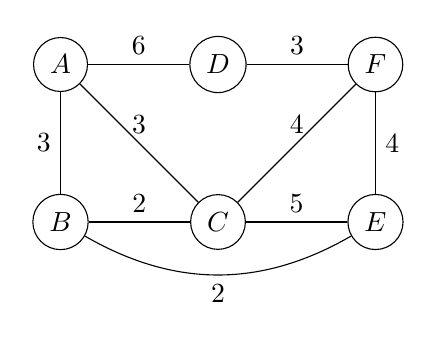
\begin{tikzpicture}[node distance = 2cm]
    \node[draw, circle] (A) {\fns\(A\)};
    \node[draw, circle, below of = A] (B) {\fns\(B\)};
    \foreach \i\j in {B/C, A/D, C/E, D/F} {
      \node[draw, circle, right of = \i] (\j) {\fns\(\j\)};
    }
    \draw[] (A) edge node[left] {\(3\)} (B);
    \foreach \i\j\k in {A/C/3, A/D/6, B/C/2, D/F/3, C/F/4, C/E/5} {
      \draw[] (\i) edge node[above] {\(\k\)} (\j);
    }
    \draw[] (E) edge node[right] {\(4\)} (F);
    \draw[] (B) edge[bend right] node[below] {\(2\)} (E);
  \end{tikzpicture}
\end{center}
\begin{choices}
  \CorrectChoice \(\{A,C\},\{C,B\},\{B,E\},\{C,F\},\{F,D\}\)
  \CorrectChoice \(\{A,B\},\{B,C\},\{B,E\},\{C,F\},\{F,D\}\)
  \choice \(\{A,C\},\{C,B\},\{C,F\},\{B,E\},\{F,D\}\)
  \CorrectChoice \(\{A,B\},\{B,E\},\{B,C\},\{E,F\},\{F,D\}\)
\end{choices}

\part[3] Which of the following statements is/are true?
\begin{choices}
  \choice The time complexity of the Prim's algorithm with a Fibonacci heap is always asymptotically better than that with a binary heap.
  \choice The time complexity of the Prim's algorithm using adjacency list and binary heap is always better than that using adjacency matrix without a priority queue.
  \CorrectChoice The minimum spanning tree of a graph is unique if all the edges have distinct weights.
  \choice The time complexity of the Kruskal's algortihm is \(O\left(|E|\alpha\left(|V|\right)\right)\) if we use the disjoint-sets with union-by-rank optimization and path-compression optimization.
  \choice If \(T\) is a minimum spanning tree obtained by performing the Prim's algorithm starting with vertex \(v\), then for any vertex \(u\) the path on the tree \(T\) connecting \(u\) and \(v\) is the shortest path from \(u\) to \(v\) in the graph.
\end{choices}

\part[3] How many different minimum spanning trees does the following graph have?
\begin{center}
  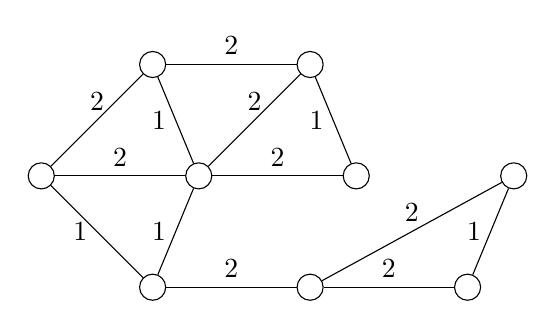
\begin{tikzpicture}[node distance = 2cm]
    \node[draw, circle] (A) {};
    \node[draw, circle, below left of = A] (B) {};
    \node[draw, circle, below right of = B] (D) {};
    \foreach \i\j in {B/C, A/E, C/F, D/G, G/H, F/I} {
      \node[draw, circle, right of = \i] (\j) {};
    }
    \foreach \i\j in {A/E, A/B, C/E, B/C, C/F, D/G, G/H, G/I} {
      \draw[] (\i) edge node[above] {\(2\)} (\j);
    }
    \foreach \i\j in {A/C, E/F, B/D, C/D, H/I} {
      \draw[] (\i) edge node[left] {\(1\)} (\j);
    }
  \end{tikzpicture}
\end{center}
\begin{oneparchoices}
  \choice \(4\)
  \choice \(5\)
  \CorrectChoice \(6\)
  \choice \(7\)
\end{oneparchoices}

\part[3] Suppose \(G=(V,E)\) is an undirected connected graph and that \(T\) is a minimum spanning tree of \(G\). Define \(w(e)\) to be the weight of \(e\) for \(e\in E\). Which of the following statements is/are true?
\begin{choices}
  \CorrectChoice If \(C\subseteq E\) is a cycle in \(G\) and \(e\in C\) is an edge on the cycle such that
  \[\forall f\in C\setminus\{e\},\quad w(e)>w(f),\]
  then \(e\) does not belong to \(T\).
  \CorrectChoice Let \(V=X\cup Y\) be a partition of \(V\) such that \(X\cap Y=\varnothing\). Define
  \[C(X,Y)=\left\{\{u,v\}\in E\mid u\in X,v\in Y\right\}.\]
  If \(e\in C(X,Y)\) is an edge such that
  \[\forall f\in C(X,Y)\setminus\{e\},\quad w(e)<w(f),\]
  then \(e\) must belong to \(T\).
  \choice Suppose \(T^\prime\neq T\) is another minimum spanning tree of \(G\). Let \(w_0\in\left\{w(e)\mid e\in T\right\}\) be the weight of some edge in \(T\). Let \(m\) be the number of edges weighted \(w_0\) in \(T\). Then \(T^\prime\) may contain less than \(m\) edges weighted \(w_0\).
  \choice If \(e\in E\) is an edge that has the largest weight among all edges in \(E\), then \(e\) cannot belong to \(T\).
\end{choices}

\end{parts}